\documentclass[12pt, a4paper]{article}

% ── Packages ──────────────────────────────────────────────────────────────────
\usepackage{amsmath, amssymb, amsthm}
\usepackage{geometry}
\usepackage{booktabs}
\usepackage{array}
\usepackage{hyperref}
\usepackage{xcolor}
\usepackage{tcolorbox}
\usepackage{enumitem}
\usepackage{parskip}
\usepackage{tikz}
\usetikzlibrary{arrows.meta, positioning, calc}

\geometry{margin=2.5cm}

% ══════════════════════════════════════════════════════════════════════════════
% ── Student-mode switch ───────────────────────────────────────────────────────
\newif\ifstudentmode
\studentmodefalse

\ifx\studentflag\undefined
\else
  \studentmodetrue
\fi
% ══════════════════════════════════════════════════════════════════════════════

% ── Student-mode macros ───────────────────────────────────────────────────────
\newcommand{\sol}[2][6cm]{%
  \ifstudentmode
    \underline{\hspace{#1}}%
  \else
    {#2}%
  \fi
}

\newcommand{\soleq}[2][3cm]{%
  \ifstudentmode
    \par\vspace{4pt}%
    \noindent\rule{\linewidth}{0.5pt}\\[#1]%
    \noindent\rule{\linewidth}{0.5pt}%
    \par\vspace{4pt}%
  \else
    \[#2\]%
  \fi
}
% ──────────────────────────────────────────────────────────────────────────────

% ── Colors & boxes ────────────────────────────────────────────────────────────
\definecolor{mainblue}{RGB}{30, 100, 180}
\definecolor{boxbg}{RGB}{235, 243, 255}
\definecolor{notebg}{RGB}{255, 248, 230}
\definecolor{warnbg}{RGB}{255, 235, 235}
\definecolor{greenbg}{RGB}{230, 255, 235}
\definecolor{purplebg}{RGB}{245, 235, 255}

\tcbuselibrary{skins, breakable}

\newtcolorbox{resultbox}{
  colback=boxbg, colframe=mainblue,
  boxrule=1.2pt, arc=4pt,
  title={Result},
  fonttitle=\bfseries\color{white},
  coltitle=white, attach boxed title to top left={yshift=-2mm, xshift=4mm},
  boxed title style={colback=mainblue, arc=3pt}
}

\newtcolorbox{notebox}{
  colback=notebg, colframe=orange!70!black,
  boxrule=1pt, arc=4pt,
  left=4pt, right=4pt
}

\newtcolorbox{warnbox}{
  colback=warnbg, colframe=red!60!black,
  boxrule=1pt, arc=4pt,
  left=4pt, right=4pt
}

\newtcolorbox{stepbox}[1]{
  colback=greenbg, colframe=green!50!black,
  boxrule=1pt, arc=4pt,
  title={#1},
  fonttitle=\bfseries,
  coltitle=green!30!black
}

\newtcolorbox{adambox}{
  colback=purplebg, colframe=purple!60!black,
  boxrule=1.4pt, arc=4pt,
  title={Adam Update Rule},
  fonttitle=\bfseries\color{white},
  coltitle=white, attach boxed title to top left={yshift=-2mm, xshift=4mm},
  boxed title style={colback=purple!70!black, arc=3pt}
}
% ──────────────────────────────────────────────────────────────────────────────

% ── Theorem environments ───────────────────────────────────────────────────────
\theoremstyle{definition}
\newtheorem{example}{Example}[section]

% ── Math macros ───────────────────────────────────────────────────────────────
\newcommand{\yhat}{\hat{y}}
\newcommand{\bW}{\mathbf{W}}
\newcommand{\pd}[2]{\dfrac{\partial #1}{\partial #2}}

% ── Document ──────────────────────────────────────────────────────────────────
\begin{document}

\begin{center}
  {\LARGE \textbf{Section 3.5: Adam}} \\[0.3em]
  {\large\itshape A Smarter Way to Update Weights} \\[0.5em]
  {\large AI Class --- Lecture Notes}%
  \ifstudentmode
    \quad {\normalsize\color{gray}[Student Copy]}%
  \fi
\end{center}

\vspace{1em}
\hrule
\vspace{1.5em}

% ══════════════════════════════════════════════════════════════════════════════
\section{Two Problems with Plain Gradient Descent}

Plain gradient descent works, but it has two frustrating properties in
practice.

\subsection*{Problem 1 — One learning rate for every weight}

The same $\eta$ is applied to every weight, regardless of how large or small
its gradient is.  Consider two weights in the same network:

\begin{center}
\renewcommand{\arraystretch}{1.3}
\begin{tabular}{llll}
\toprule
Weight & Gradient $g$ & GD step ($\eta=0.1$) & Problem \\
\midrule
$w_A$ & $-0.002$ & $+0.0002$ & Barely moves --- too slow \\
$w_B$ & $-5.000$ & $+0.500$  & May overshoot --- too fast \\
\bottomrule
\end{tabular}
\end{center}

A single global $\eta$ that is safe for $w_B$ is painfully slow for $w_A$,
and one that is fast enough for $w_A$ will cause $w_B$ to diverge.

\subsection*{Problem 2 — Oscillation in steep directions}

If the loss surface is much steeper in one direction than another, gradient
descent zigzags across the steep axis while crawling along the shallow one:

\begin{center}
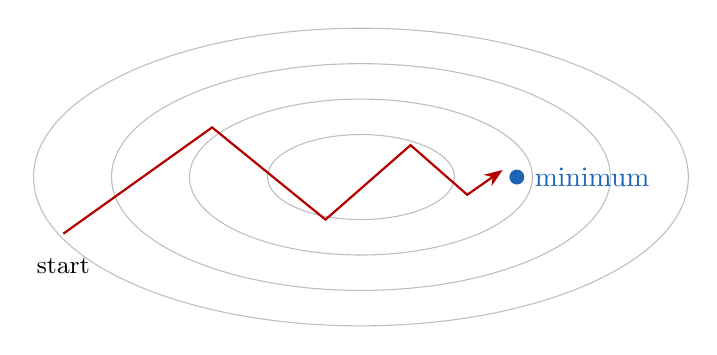
\begin{tikzpicture}[scale=0.9, >=Stealth]
  % Elliptical contours
  \foreach \r in {0.6, 1.1, 1.6, 2.1} {
    \draw[gray!50, thin] (0,0) ellipse ({\r*2.2} and \r);
  }
  % Zigzag path
  \draw[thick, red!70!black, ->]
    (-4.2, -0.8) -- (-2.1, 0.7) -- (-0.5, -0.6)
    -- (0.7, 0.45) -- (1.5, -0.25) -- (2.0, 0.1);
  % Minimum
  \fill[mainblue] (2.2, 0) circle (3pt) node[right=3pt] {minimum};
  % Axes
  \node[below] at (-4.2,-1.0) {\small start};
\end{tikzpicture}
\end{center}

\textbf{Adam} (Adaptive Moment Estimation) fixes both problems with two ideas:
momentum and adaptive step sizes.

% ══════════════════════════════════════════════════════════════════════════════
\section{Idea 1 — Momentum (the $m$ term)}

Instead of using the raw gradient at each step, keep a \textbf{running
average} of recent gradients, called the \textbf{first moment} $m_t$:

\[
  m_t = \beta_1 \, m_{t-1} + (1 - \beta_1)\, g_t
\]

where $g_t = \partial J / \partial w$ at step $t$, and $\beta_1 = 0.9$ by
default.

Think of it as a weighted memory: $m_t$ is $90\%$ of what was accumulated
before, plus $10\%$ of the new gradient.

\begin{center}
\renewcommand{\arraystretch}{1.3}
\begin{tabular}{lp{9cm}}
\toprule
Situation & Effect on $m_t$ \\
\midrule
Gradient keeps the same sign (steady slope) &
  $m_t$ grows large $\Rightarrow$ the update \emph{accelerates}, like a
  ball rolling downhill. \\
Gradient alternates sign (oscillation) &
  Positive and negative values cancel out $\Rightarrow$ $m_t$ stays small,
  damping the zigzag. \\
\bottomrule
\end{tabular}
\end{center}

% ══════════════════════════════════════════════════════════════════════════════
\section{Idea 2 --- Adaptive Step Sizes (the $v$ term)}

Keep a running average of the \textbf{squared} gradient, called the
\textbf{second moment} $v_t$:

\[
  v_t = \beta_2 \, v_{t-1} + (1 - \beta_2)\, g_t^2
\]

with $\beta_2 = 0.999$ by default.
Because we square $g_t$, the sign is gone --- $v_t$ measures
\emph{how large} gradients have been recently.

The update then \textbf{divides by $\sqrt{v_t}$}:

\begin{center}
\renewcommand{\arraystretch}{1.3}
\begin{tabular}{lcp{6cm}}
\toprule
History of $g$ & $v_t$ & Effective step \\
\midrule
Consistently large & Large & $\propto 1/\sqrt{\text{large}}$ = small
  $\Rightarrow$ pulls back weights with big gradients \\
Consistently small & Small & $\propto 1/\sqrt{\text{small}}$ = large
  $\Rightarrow$ pushes forward weights with tiny gradients \\
\bottomrule
\end{tabular}
\end{center}

Every weight gets its own \emph{effective} learning rate, automatically tuned
by its recent gradient history.

% ══════════════════════════════════════════════════════════════════════════════
\section{The Adam Update Rule}

Combining momentum and adaptive step sizes, and adding a small
\textbf{bias correction} (explained below):

\begin{adambox}
At each training step $t$, for each weight $w$ with gradient $g_t$:

\vspace{0.5em}
\textbf{Update the running averages:}
\begin{align*}
  m_t &= \beta_1 \, m_{t-1} + (1-\beta_1)\, g_t \\
  v_t &= \beta_2 \, v_{t-1} + (1-\beta_2)\, g_t^2
\end{align*}

\textbf{Apply bias correction:}
\[
  \hat{m}_t = \frac{m_t}{1 - \beta_1^t},
  \qquad
  \hat{v}_t = \frac{v_t}{1 - \beta_2^t}
\]

\textbf{Update the weight:}
\[
  w \;\longleftarrow\; w - \eta \,\frac{\hat{m}_t}{\sqrt{\hat{v}_t} + \varepsilon}
\]

\textbf{Default hyperparameters:}
$\eta = 0.001,\quad \beta_1 = 0.9,\quad \beta_2 = 0.999,\quad
\varepsilon = 10^{-8}$.
\end{adambox}

\vspace{0.5em}

$\varepsilon$ is a tiny constant added to prevent division by zero when
$\hat{v}_t \approx 0$.

\begin{notebox}
\textbf{Why bias correction?}
At the start ($t = 1$), $m_0 = 0$ and $v_0 = 0$ --- the running averages
are initialised at zero and are therefore biased too low.
Dividing by $(1 - \beta^t)$ compensates: at $t=1$ it divides by $(1-0.9) = 0.1$,
scaling the average back up to reflect the single gradient seen so far.
After many steps $\beta^t \approx 0$, so the correction disappears and the
raw averages are used directly.
\end{notebox}

% ══════════════════════════════════════════════════════════════════════════════
\section{Hand-Calculated Example}

We use the gradient $g_1 = \partial J / \partial w^{(2)}_1 = -0.084$
computed in Section 3.4 for the first training step ($t = 1$).
Both running averages start at zero: $m_0 = 0$, $v_0 = 0$.

% ──────────────────────────────────────────────────────────────────────────────
\begin{stepbox}{Step 1 \quad Update the running averages}
\begin{align*}
  m_1 &= 0.9 \times 0 + 0.1 \times (-0.084)
       = \sol[4cm]{-0.0084} \\[6pt]
  v_1 &= 0.999 \times 0 + 0.001 \times (-0.084)^2
       = 0.001 \times 0.007056
       = \sol[4cm]{7.056 \times 10^{-6}}
\end{align*}
\end{stepbox}

\vspace{0.8em}

% ──────────────────────────────────────────────────────────────────────────────
\begin{stepbox}{Step 2 \quad Apply bias correction ($t = 1$)}
\begin{align*}
  \hat{m}_1 &= \frac{m_1}{1 - 0.9^1}
             = \frac{-0.0084}{0.1}
             = \sol[4cm]{-0.084} \\[6pt]
  \hat{v}_1 &= \frac{v_1}{1 - 0.999^1}
             = \frac{7.056 \times 10^{-6}}{0.001}
             = \sol[4cm]{7.056 \times 10^{-3}}
\end{align*}
\end{stepbox}

\vspace{0.8em}

% ──────────────────────────────────────────────────────────────────────────────
\begin{stepbox}{Step 3 \quad Update the weight}

\[
  \sqrt{\hat{v}_1} = \sqrt{7.056 \times 10^{-3}}
                   = \sol[3cm]{0.084}
\]

\[
  w^{(2)}_1 \;\longleftarrow\;
  0.5 - 0.001 \times \frac{-0.084}{0.084 + 10^{-8}}
  \approx 0.5 - 0.001 \times (-1.000)
  = \sol[3cm]{0.501}
\]
\end{stepbox}

\vspace{0.5em}

\begin{notebox}
\textbf{A clean pattern at $t = 1$.}
The bias correction at the first step recovers $\hat{m}_1 = g_1$ (the raw
gradient) and $\sqrt{\hat{v}_1} = |g_1|$ (the absolute gradient).  The
effective step is therefore:
\[
  \eta \times \frac{g_1}{|g_1|} = \eta \times \operatorname{sign}(g_1)
  = \pm\, 0.001.
\]
At step 1, Adam always takes a step of exactly $\pm\eta$, regardless of how
large or small the gradient is.  The gradient magnitude starts shaping the
step only as $v_t$ accumulates history over multiple steps.
\end{notebox}

% ──────────────────────────────────────────────────────────────────────────────
\subsection*{Comparison with plain gradient descent}

\begin{center}
\renewcommand{\arraystretch}{1.4}
\begin{tabular}{lcc}
\toprule
 & Plain GD ($\eta = 0.1$) & Adam ($\eta = 0.001$) \\
\midrule
Gradient $g_1$ & $-0.084$ & $-0.084$ \\
Weight before  & $0.500$  & $0.500$ \\
Update size    & $0.1 \times 0.084 = 0.0084$ & $0.001$ \\
Weight after   & $0.508$  & $0.501$ \\
\bottomrule
\end{tabular}
\end{center}

The step sizes differ because the two methods use different $\eta$ values.
The key advantage of Adam is not the size of this first step but that the
effective step size \emph{adapts} to each weight's gradient history ---
it neither stalls on weights with tiny gradients nor explodes on weights
with large ones.

% ══════════════════════════════════════════════════════════════════════════════
\section{Why Adam Is the Default Choice}

\begin{center}
\renewcommand{\arraystretch}{1.3}
\begin{tabular}{lll}
\toprule
Property & Plain GD & Adam \\
\midrule
Learning rate to tune & One global $\eta$ & One global $\eta$ (but less sensitive) \\
Per-weight step size  & Same for all & Adapts to gradient history \\
Handles oscillation   & No  & Yes (momentum cancels zigzags) \\
Handles sparse gradients & Poorly & Well (small $v$ → large effective step) \\
Default $\eta$        & Problem-specific & $0.001$ usually works \\
\bottomrule
\end{tabular}
\end{center}

\begin{warnbox}
\textbf{Adam is not magic.}
It still requires choosing $\eta$, and it can overfit faster than plain GD
in some settings.  For problems where generalisation matters most, simpler
optimisers (SGD with momentum) are sometimes preferred.  Adam is, however,
the best default starting point for most deep learning applications.
\end{warnbox}

% ══════════════════════════════════════════════════════════════════════════════
\section{The Complete Training Loop}

Putting everything from Sections 3.2--3.5 together:

\vspace{0.5em}
\begin{center}
\renewcommand{\arraystretch}{1.5}
\begin{tabular}{cl}
\toprule
Step & Action \\
\midrule
1 & Initialise all weights randomly; set $m = 0$, $v = 0$, $t = 0$. \\
2 & For each training example (or mini-batch): \\
  & \quad (a) \textbf{Forward pass} --- compute $\yhat$ and $J$. \\
  & \quad (b) \textbf{Backpropagation} --- compute $\partial J/\partial w$
              for every weight. \\
  & \quad (c) \textbf{Adam update} --- update $m$, $v$, then $w$. \\
  & \quad (d) Increment $t$. \\
3 & Repeat Step 2 until $J$ is small enough or a maximum number of \\
  & epochs is reached. \\
\bottomrule
\end{tabular}
\end{center}

\end{document}
